% autore: Matilde Padovano

Inanzitutto dobbiamo costruire un grafo, dove collego ogni capo ai suoi dipendenti, perciò collego, per ogni dipendente $i$,  $C[i]$ a $i$. \itemize
Ora per risolvere questo problema è sufficiente fare due osservazioni:\itemize \newline
⦁
\item Se prendo una persona $x$ in squadra, di sicuro non posso prendere nessuno dei suoi dipendenti(diretti o indiretti).\newline

\item Se non prendo una persona $x$ in squadra, posso decidere per ogni dipendente diretto se  prenderlo o non prenderlo.\newline

A questo punto è facile notare che basta lanciare una dfs dal presidente, e a ogni nodo decidere se conviene fermarsi(prendendo la bravura del nodo corrente) o proseguire( prendendo la somma delle soluzioni ottimali per ogni nodo figlio).\itemize
\newline

\colorbox{white}{\makebox[.99\textwidth][l]{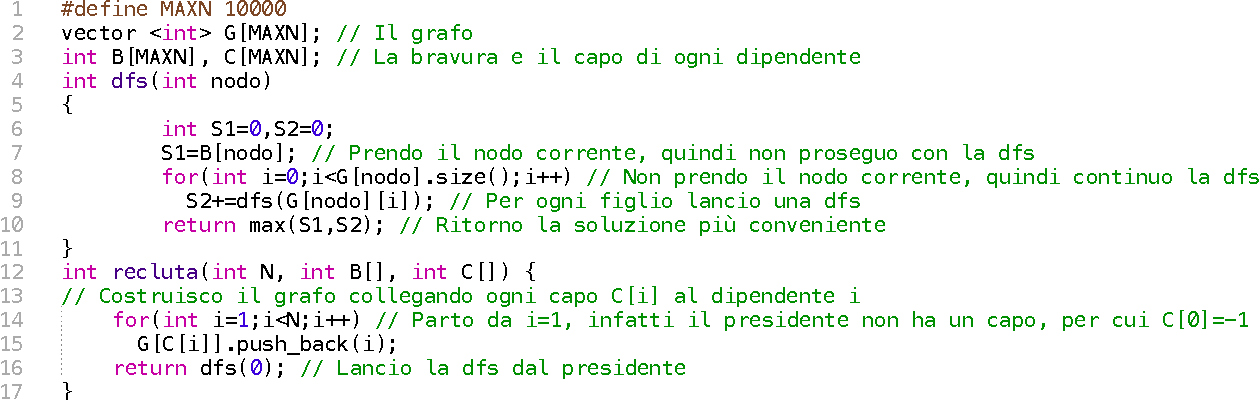
\includegraphics[scale=.8]{rugby.pdf}}} 
